
\documentclass{beamer}
\setbeamertemplate{navigation symbols}{}


\usetheme{Madrid}
%\usetheme{AnnArbor}
%\usetheme{Warsaw}
%\usetheme{CambridgeUS}

%\usecolortheme{albatross}
%\usecolortheme{beaver}
\usecolortheme{beetle}
%\usecolortheme{spruce}

\beamersetuncovermixins{\opaqueness<1>{25}}{\opaqueness<2->{15}}

 \usepackage{array}
 \usepackage{amssymb}
 \usepackage{theorem}
 \usepackage{fancyvrb}%  extended verbatim environments
  \fvset{fontsize=\footnotesize,xleftmargin=2em}

\usepackage{graphicx,psfrag,pstricks,cite,amsmath,amssymb,latexsym}

\graphicspath{{./Figures/}}



\DeclareRobustCommand{\gumstix}{Gumstix\textsuperscript{\textregistered}}
\DeclareRobustCommand{\overo}{Overo\textsuperscript{\textregistered}}
\DeclareRobustCommand{\tobi}{Tobi~}
\DeclareRobustCommand{\pinto}{Pinto~}
\DeclareRobustCommand{\garmin}{Garmin\textsuperscript{TM}}
\DeclareRobustCommand{\houston}{Houston RADAR\textsuperscript{TM}}
\DeclareRobustCommand{\ICE_T}{\textcolor{Blue}{ICE-T}}
\DeclareRobustCommand{\UXAS}{\textcolor{Blue}{UxAS}}






\begin{document}
\title[Area Monitoring using UAV and UGS]{Development and Flight Test of an Area Monitoring System Using Unmanned Aerial Vehicles and Unattended Ground Sensors}  
\author{Steven Rasmussen and Derek Kingston}
%\date{\today} 
\date{June 12, 2015} 


\begin{frame}
\titlepage
\end{frame}

\begin{frame}\frametitle{Table of contents}
%\tableofcontents[pausesections]
\tableofcontents
\end{frame} 

\section{UAV Autonomy} 
\begin{frame}\frametitle{UAV Autonomy} 
\begin{itemize}
%\item Autonomous agents perceive, decide, and act on their own.
\item In order to accomplish a task autonomously, a UAV must have access to \emph{actionable sensed information}.\\
%\item Enabling technologies are either assumed to exist or the tasks have been simplified to accommodate autonomous decision making
\item  \emph{Actionable information} is UAV understandable data that the UAV can use to decide on the course of actions that it must perform to accomplish an assigned mission. \\
\item The information must be \emph{sensed} in order to make it possible for the UAV to get updated measurements for the task.\\
%\item A number of different sensor modalities have been amenable to exploitation.
\item With the ability to collect actionable sensed information the UAV is able to:
\begin{itemize}
\item take some measure of the environment
\item develop a plan to perform a desired task
\item execute the plan using updates from the sensor, as feedback, during the task execution.
\end{itemize}
\end{itemize}
\end{frame}


\section{A Combined UAV/UGS System} 
\begin{frame}\frametitle{A Combined UAV/UGS System} 
\emph{System Goal:} explore a combined UAV/UGS system that autonomously detects intrusions on a road network and delivers imagery of potential threats only when that imagery has a high likelihood of containing an intruder
\begin{itemize}
\item Many current UGS systems are placed carefully and have line-of-sight to other UGSs or to a “gateway” node.
\item Each UGS operates completely independently and has no mechanism to report alarms to a centralized base location. 
\item A UAV must query the UGS when in range to download the stored intrusion detections.
\item Based on that information, the UAV collects and stores onboard relevant video clips for future delivery to a human operator for analysis.
\end{itemize}
\end{frame}

\section{Autonomous UAV/UGS Area Monitoring Development} \label{sec:hardware}
\begin{frame}\frametitle{Autonomous UAV/UGS Area Monitoring Development} 
%
\begin{itemize}
\item In order to implement an effective UAV/UGS monitoring system, both software and hardware components were designed, implemented, tested, and fielded.\\
\item Because of it's small size, processing capability, and the ability to integrate it into our design, we choose the \overo ~family of embedded processors to act as both the on-board and UGS computers.
\end{itemize}
\end{frame}



%\subsection{UAV On-Board Processor}
\begin{frame}\frametitle{UAV On-Board Processor} 
\begin{figure}
\centering
      \includegraphics[width=0.8\textwidth]{OnBoardProcessorLayout}
      \label{fig:OnBoardProcessorLayout}
\end{figure}
\end{frame}
%\subsection{UGS Design/Operation}
\begin{frame}\frametitle{UGS Design/Operation} 
\begin{figure}
\centering
      \includegraphics[width=0.8\textwidth]{UgsHardwareLayout}
      \label{fig:UgsHardwareLayout}
\end{figure}
\end{frame}
%\subsection{UAV/UGS Communication}
\begin{frame}\frametitle{UAV/UGS Communication} 
\begin{table}
\begin{flushleft}
\begin{tabular}{|m{1.0cm}|m{1.0cm}|m{8.25cm}|}\hline
 \textbf{FROM}  & \textbf{TO}     & \textbf{MESSAGE}\\ \hline \hline
UAV & UGS & \emph{HeartbeatMessage} - Send Heartbeat over multicast channel.\\ \hline
UGS & UAV & \emph{HeartbeatResponse} - Send response to heartbeat message as TCP/IP client\\ \hline
UAV & UGS & \emph{MessageQuery} - Ask for all messages since last contact.\\ \hline
UGS & UAV & \emph{QueryResponse} - Send list of all messages being sent.\\ \hline
UGS & UAV & \emph{IntruderAlert, DismountMessage} - send all messages that match the query.\\ \hline
UAV & UGS & \emph{VicsAck} - Send an acknowledgement for each message received.\\ \hline
\end{tabular}
\end{flushleft}
\end{table}
\end{frame}


\section{ICE-T Autonomous UAV/UGS Area Monitoring Architecture}
\begin{frame}\frametitle{Autonomous UAV/UGS Area Monitoring Development} 
\begin{figure}
\centering
      \includegraphics[width=0.9\textwidth]{AreaMonitoringArchitecture}
      \label{fig:AreaMonitoringArchitecture}
\end{figure}
\end{frame}
%\subsection{Messages}
%\subsection{Ground Station}
%\subsection{PCC}
%\subsection{Piccolo}
%\subsection{On-Board Processor}
%\subsection{Dismount}
\section{Simulating UAV/UGS Scenarios\label{sec:Simulation}}
\begin{frame}\frametitle{AMASE UAV/UGS Simulation Snapshot} 
\begin{figure}[htb]
\centering
      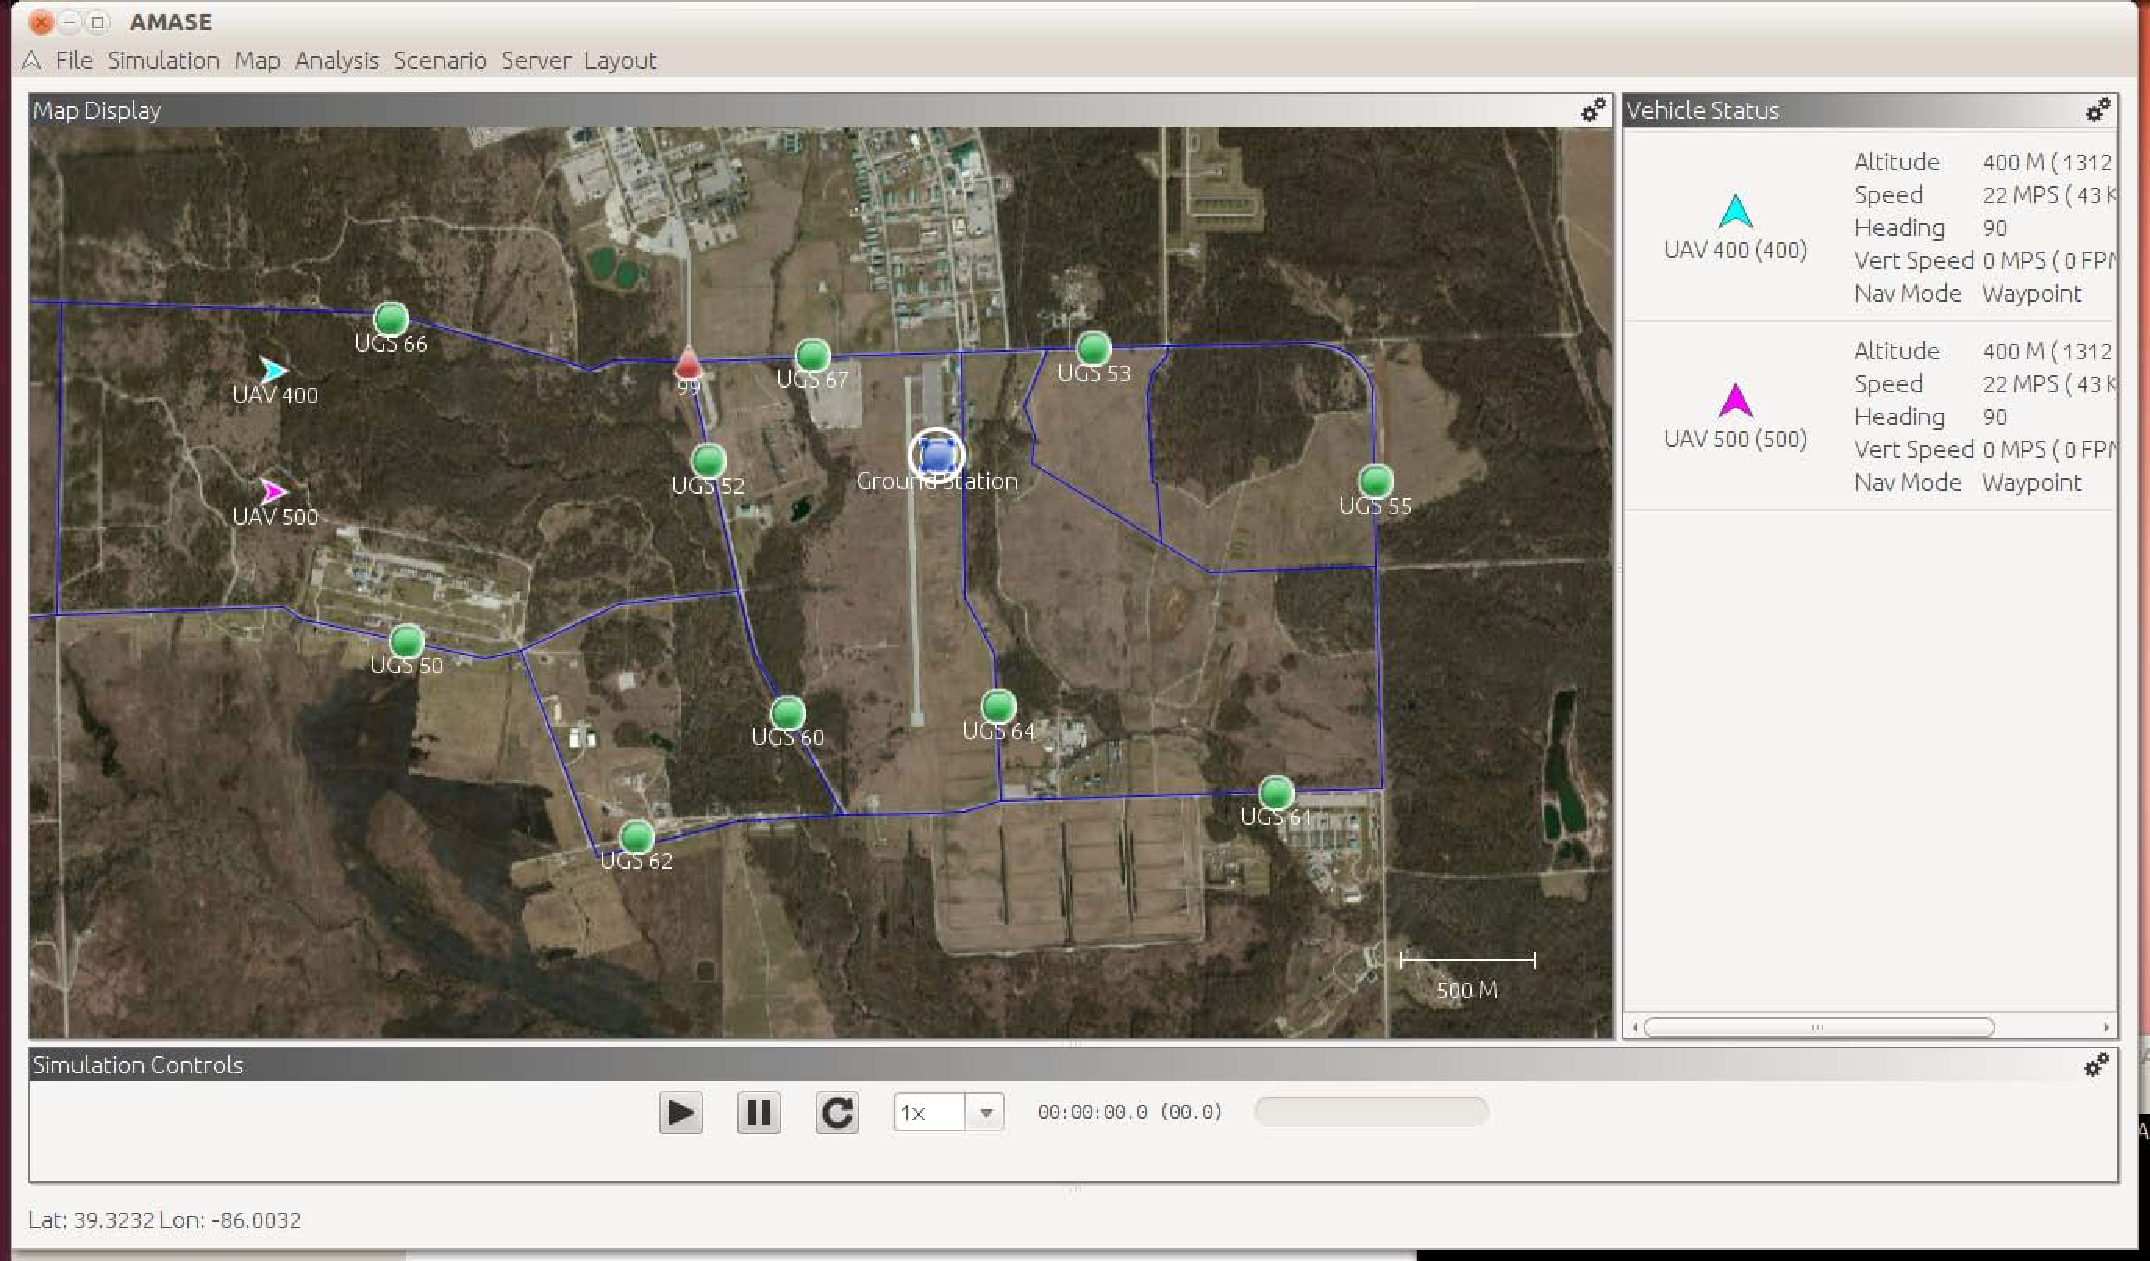
\includegraphics[width=0.7\textwidth]{AMASE_UGS_Scenario}
\end{figure}
\end{frame}

\section{Flight Testing/Demonstration\label{sec:FlightTest}}
\begin{frame}\frametitle{All of the UGS constructed for the exercise.} 
\begin{figure}[htb]
\centering
      \includegraphics[width=0.8\textwidth]{AllUgs}
\end{figure}
\end{frame}

\begin{frame}\frametitle{UGS Placement for flight tests.} 
\begin{figure}[htb]
\centering
      \includegraphics[width=0.8\textwidth]{UgsPlacement_02a}
\end{figure}
\end{frame}

\begin{frame}\frametitle{Intruder alert tracks for a 30 minute time window.} 
\begin{figure}[htb]
\centering
      \includegraphics[width=0.8\textwidth]{UGS_Tracks30MinWindow_01}
\end{figure}
\end{frame}

\begin{frame}\frametitle{UGS patrol flight path, based on operator selected waypoints.} 
\begin{figure}[htb]
\centering
      \includegraphics[width=0.8\textwidth]{UgsMonitoringPath_02}
\end{figure}
\end{frame}

\begin{frame}\frametitle{UGS patrol plan, generated on-board the UAV.} 
\begin{figure}[htb]
\centering
      \includegraphics[width=0.8\textwidth]{UgsPatrolPlan}
\end{figure}
\end{frame}

\begin{frame}\frametitle{UAV road search plans, generated on-board the UAV.} 
\begin{figure}[htb]
\centering
      \includegraphics[width=0.8\textwidth]{RoadSearchPlans_02}
\end{figure}
\end{frame}

\section{At A Glance}
\begin{frame}\frametitle{At A Glance} 
\begin{itemize}
\item \textbf{UGS Deployed:} \emph{31}
\item \textbf{Deployment Area:} \emph{35km X 60km}
\item \textbf{UGS Setup Time:} \emph{2 days}
\item \textbf{UGS Deployment Time:} \emph{2 weeks}
\item \textbf{Time Synchronization:} \emph{GPS}
\item \textbf{Total Intruder Alerts Generated:} \emph{53,000}
\item \textbf{Percentage of True Alerts:} \emph{30\%}
\item \textbf{Number Alerts Collected by UAV:} \emph{4300 (8\% of total)}
\item \textbf{Number Alerts Sent to GCS from UAV:} \emph{240}
\end{itemize}
\end{frame}

\section{Questions?}
\begin{frame}\frametitle{} 
\begin{center}
\Huge Questions?
\end{center}
\end{frame}


\end{document}